\documentclass{article}
\usepackage{fontspec, xunicode, xltxtra} 
\setmainfont{Microsoft YaHei} 
\usepackage{setspace}
\usepackage{ctex} 
\usepackage{geometry}
\usepackage[Glenn]{fncychap}
\usepackage{listings}
\usepackage{color}
\usepackage{verbatim}
\usepackage{fancyhdr}


\newfontfamily\monaco{Monaco}

\definecolor{dkgreen}{rgb}{0,0.6,0}
\definecolor{gray}{rgb}{0.5,0.5,0.5}
\definecolor{mauve}{rgb}{0.58,0,0.82}

\geometry{left=2.5cm,right=1.7cm,top=1.0cm,bottom=1.5cm}

\lstset{
    frame=simple,
    language=c++,
    aboveskip=3mm,
    belowskip=3mm,
    showstringspaces=false,
    basicstyle=\monaco,
    numbers=none,
    numberstyle=\tiny\color{gray},
    keywordstyle=\bfseries\monaco,%\fontspec{monaco Bold}\bfseries,
    commentstyle=\color{dkgreen},
    stringstyle=\color{mauve},
    breaklines=true,
    breakatwhitespace=true,
    tabsize=4,
    numbers = left,
}

\begin{document}

\begin{titlepage}

\thispagestyle{empty}
\pagebreak
\pagestyle{plain}
\tableofcontents
\end{titlepage}


%-------------------------基本操作-----------------
\section{基本操作}

\subsection{离散化}
\subsubsection{一维线离散化}
\lstinputlisting{基本操作/离散化/一维线离散化.cpp}
\subsubsection{二维点离散化}
\lstinputlisting{基本操作/离散化/二维点离散化.cpp}

\subsection{矩阵快速幂}
\lstinputlisting{基本操作/矩阵快速幂.cpp}

\subsection{二进制枚举}
\lstinputlisting{基本操作/二进制枚举.cpp}

\subsection{状态压缩}
\lstinputlisting{基本操作/状态压缩.cpp}

\subsection{bitset}
\lstinputlisting{基本操作/bitset.cpp}


%------------------------数论----------------
\section{数论}

\subsection{快速幂}
\lstinputlisting{数论/快速幂.cpp}

\subsection{快速乘(×)龟速乘(√)}
\lstinputlisting{数论/快速乘.cpp}

\subsection{中国剩余定理}
\subsubsection{模数不互质(扩展中国剩余)}
\lstinputlisting{数论/中国剩余定理/模数不互质(扩展中国剩余).cpp}
\subsubsection{模数互质}
\lstinputlisting{数论/中国剩余定理/模数互质.cpp}

\subsection{博弈论}
\subsubsection{Bash博弈}
\lstinputlisting{数论/博弈论/Bash博弈.cpp}
\subsubsection{威佐夫博弈}
\lstinputlisting{数论/博弈论/威佐夫博弈.cpp}
\subsubsection{威佐夫博弈扩展}
\lstinputlisting{数论/博弈论/威佐夫博弈扩展.cpp}
\subsubsection{Nim博弈}
\lstinputlisting{数论/博弈论/Nim博弈.cpp}
\subsubsection{非常规}
\begin{figure}[htb] 
 \center{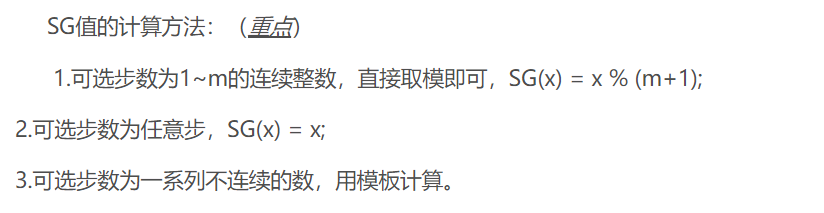
\includegraphics[width=15cm]  {数论/博弈论/非常规_pic.png}} 
 \end{figure}
\lstinputlisting{数论/博弈论/非常规.cpp}

\subsection{素数}
\subsubsection{素数检测(米勒罗宾)}
\lstinputlisting{数论/素数/素数检测(米勒罗宾).cpp}
\subsubsection{素数线性筛}
\lstinputlisting{数论/素数/素数线性筛.cpp}
\subsubsection{区间筛}
\lstinputlisting{数论/素数/区间筛.cpp}

\subsection{合数}
\subsubsection{合数分解}
\lstinputlisting{数论/合数/合数分解.cpp}
\subsubsection{区间合数分解}
\lstinputlisting{数论/合数/区间合数分解.cpp}
\subsubsection{阶乘的因数个数}
\lstinputlisting{数论/合数/阶乘的因数个数.cpp}
\subsubsection{组合数的质因数个数}
\lstinputlisting{数论/合数/组合数的质因数个数.cpp}
\subsubsection{约数之和}
\lstinputlisting{数论/合数/约数之和.cpp}

\subsection{求逆元}
\subsubsection{模数为质数}
\lstinputlisting{数论/求逆元/模数为质数.cpp}
\subsubsection{模数不为质数}
\lstinputlisting{数论/求逆元/模数不为质数.cpp}
\subsubsection{线性逆元}
\lstinputlisting{数论/求逆元/线性逆元.cpp}
\subsubsection{阶乘逆元}
\lstinputlisting{数论/求逆元/阶乘逆元.cpp}

\subsection{GCD}
\subsubsection{一些性质}
\lstinputlisting{数论/GCD/一些性质.cpp}
\subsubsection{区间gcd}
\lstinputlisting{数论/GCD/区间gcd.cpp}
\subsubsection{gcd+lcm}
\lstinputlisting{数论/GCD/gcd+lcm.cpp}

\subsection{欧拉函数}
\subsubsection{单个欧拉值(sqrt(n))}
\lstinputlisting{数论/欧拉函数/单个值欧拉.cpp}
\subsubsection{线性筛欧拉}
\lstinputlisting{数论/欧拉函数/线性筛欧拉.cpp}
\subsubsection{欧拉妙用}
\lstinputlisting{数论/欧拉函数/欧拉妙用.cpp}
\subsubsection{欧拉降幂}
\lstinputlisting{数论/欧拉函数/欧拉降幂.cpp}

\subsection{扩展欧几里得}
\lstinputlisting{数论/扩展欧几里得.cpp}

\subsection{同余不等式}
\lstinputlisting{数论/同余不等式.cpp}

\subsection{高次同余方程}
\lstinputlisting{数论/高次同余方程.cpp}

\subsection{高斯消元}
\subsubsection{一般模板(double)}
\lstinputlisting{数论/高斯消元/一般模板(double).cpp}
\subsubsection{高精度java模板}
\lstinputlisting[language=Java]{数论/高斯消元/高精度java模板.java}
\subsubsection{高斯解同余方程}
\lstinputlisting{数论/高斯消元/高斯解同余方程.cpp}   

%----------------------数学---------------------
\section{数学}

\subsection{蔡勒公式(1592之后)}
\lstinputlisting{数学/蔡勒公式(1582之后).cpp} 


%----------------------字符串--------------------
\section{字符串}

\subsection{KMP}
\subsubsection{求next方法1}
\begin{figure}[htb] 
 \center{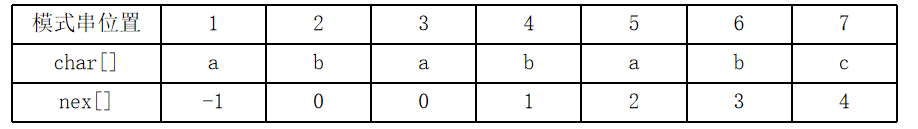
\includegraphics[width=15cm]  {字符串/KMP/求next1_pic1.png}} 
 \end{figure}
 \begin{figure}[htb] 
 \center{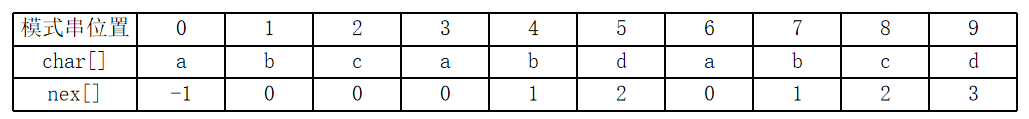
\includegraphics[width=15cm]  {字符串/KMP/求next1_pic2.png}} 
 \end{figure}
\lstinputlisting{字符串/KMP/求next1.cpp}
\subsubsection{求next方法2}
\begin{figure}[htb] 
 \center{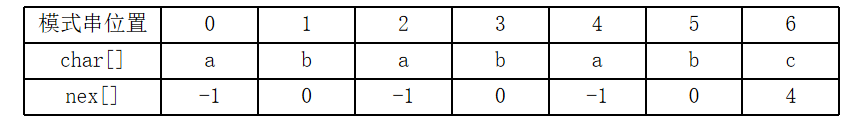
\includegraphics[width=15cm]  {字符串/KMP/求next2_pic1.png}} 
 \end{figure}
 \begin{figure}[htb] 
 \center{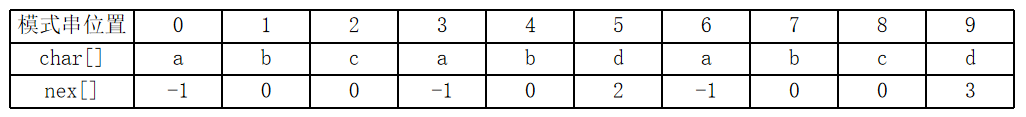
\includegraphics[width=15cm]  {字符串/KMP/求next2_pic2.png}} 
 \end{figure}
\lstinputlisting{字符串/KMP/求next2.cpp}

\subsection{字符串部分匹配}
\lstinputlisting{字符串/字符串部分匹配.cpp} 

\subsection{求字符串的前缀是否为周期串}
\lstinputlisting{字符串/求字符串的前缀是否为周期串.cpp}

\subsection{字符串由多少相同的字串组成}
\lstinputlisting{字符串/字符串由多少相同的字串组成.cpp}

\subsection{双倍回文}
\lstinputlisting{字符串/双倍回文.cpp}


%-----------------------计算几何--------------------
\section{计算几何}

\subsection{叉积}
\subsubsection{点线式}
\lstinputlisting{计算几何/叉积/点线式.cpp} 
\subsubsection{重载版}
\lstinputlisting{计算几何/叉积/重载版.cpp} 
\subsubsection{叉积算多边形面积}
\lstinputlisting{计算几何/叉积/叉积算多边形面积.cpp}

\subsection{极角排序}
\subsubsection{叉积计算}
\lstinputlisting{计算几何/极角排序/叉积计算.cpp}
\subsubsection{atan2函数计算}
\lstinputlisting{计算几何/极角排序/atan2函数计算.cpp}

\subsection{凸包}
\subsubsection{一般凸包}
\lstinputlisting{计算几何/凸包/一般凸包.cpp}
\subsubsection{最大空凸包}
\lstinputlisting{计算几何/凸包/最大空凸包.cpp}

\subsection{半平面交}
\subsubsection{叉积计算}
\lstinputlisting{计算几何/半平面交/判不等式组是否有解.cpp}
\subsubsection{半平面交存点}
\lstinputlisting{计算几何/半平面交/半平面交存点.cpp}

%-------------------------数据结构--------------------
\section{数据结构}

\subsection{单调栈+单调队列}
\subsubsection{单调栈}
\lstinputlisting{数据结构/单调栈&单调队列/单调栈.cpp}
\subsubsection{单调队列}
\lstinputlisting{数据结构/单调栈&单调队列/单调队列.cpp}

\subsection{树状数组}
\subsubsection{lowbit之和}
\lstinputlisting{数据结构/树状数组/lowbit之和.cpp}
\subsubsection{区间加减+区间和查询}
\lstinputlisting{数据结构/树状数组/区间加减&区间和查询.cpp}
\subsubsection{统计前后顺序不同数字对个数(三维偏序问题)}
\lstinputlisting{数据结构/树状数组/统计前后顺序不同数字对个数(三维偏序问题).cpp}

\subsection{ZKW线段树}
\subsubsection{开局}
\lstinputlisting{数据结构/线段树/ZKW线段树/开局.cpp}
\subsubsection{单点修改+区间查询}
\lstinputlisting{数据结构/线段树/ZKW线段树/单点修改+区间查询.cpp}
\subsubsection{单点修改+区间查询最大字段和}
\lstinputlisting{数据结构/线段树/ZKW线段树/单点修改+区间查询最大子段和.cpp}
\subsubsection{区间加减+单点查询}
\lstinputlisting{数据结构/线段树/ZKW线段树/区间加减+单点查询.cpp}
\subsubsection{区间加减+区间最值查询(lazy标记)}
\lstinputlisting{数据结构/线段树/ZKW线段树/区间加减+区间最值查询(lazy标记).cpp}

\subsection{二维线段树}
\lstinputlisting{数据结构/线段树/二维线段树/单点修改&区间查询(最值&最大值).cpp}

\subsection{普通线段树}
\subsubsection{单点修改+区间查询}
\lstinputlisting{数据结构/线段树/普通线段树/单点修改&区间查询.cpp}
\subsubsection{区间修改+区间查询}
\lstinputlisting{数据结构/线段树/普通线段树/区间修改&区间查询.cpp}
\subsubsection{区间染色}
\lstinputlisting{数据结构/线段树/普通线段树/区间染色.cpp}
\subsubsection{区间修改+区间查询:矩阵}
\lstinputlisting{数据结构/线段树/普通线段树/区间修改&区间查询_矩阵ver.cpp}


\subsection{普通平衡树Treap}
\lstinputlisting{数据结构/普通平衡树Treap.cpp}

\subsection{树链剖分}
\lstinputlisting{数据结构/树链剖分.cpp}

%-------------------------图论----------------------

\section{图论}

\subsection{前向星}
\lstinputlisting{图论/前向星.cpp}

\subsection{最短路}
\subsubsection{Dijkstra+堆优化}
\lstinputlisting{图论/最短路/Dijkstra+堆优化.cpp}
\subsubsection{SPFA(判环)}
\lstinputlisting{图论/最短路/SPFA(判环).cpp}
\subsubsection{Floyd}
\lstinputlisting{图论/最短路/Floyd.cpp}

\subsection{第K短路}
\lstinputlisting{图论/第k短路.cpp}

\subsection{最小环}
\subsubsection{Floyd}
\lstinputlisting{图论/最小环/Floyd.cpp}
\subsubsection{Dijkstra+剪枝}
\lstinputlisting{图论/最小环/Dijkstra+剪枝.cpp}

\subsection{网络流}
\subsubsection{二分图匹配}
\lstinputlisting{图论/网络流/二分图匹配.cpp}
\subsubsection{最大流}
\paragraph{Dinic}
\lstinputlisting{图论/网络流/最大流/Dinic.cpp}

\subsection{点分治}
\lstinputlisting{图论/点分治.cpp}

%-----------------------莫队--------------------
\section{莫队}

\subsection{区间查询,统计两个相同概率}
\lstinputlisting{莫队算法/区间查询,统计两个相同概率.cpp}
\subsection{时间戳+统计有多少个不同的数}
\lstinputlisting{莫队算法/时间戳+统计有多少个不同的数.cpp}
\subsection{树状数组维护区间两数之差}
\lstinputlisting{莫队算法/树状数组维护区间两数之差.cpp}
\subsection{统计有多少个不同的数}
\lstinputlisting{莫队算法/统计有多少个不同的数.cpp}
\subsection{回滚莫队}
\lstinputlisting{莫队算法/回滚莫队.cpp}

%-----------------------java------------------
\section{Java}
\subsection{开头}
\lstinputlisting[language=Java]{java/开头.java}
\subsection{加减乘除等}
\lstinputlisting[language=Java]{java/加减乘除等.java}
\subsection{Java大数二分}
\lstinputlisting[language=Java]{java/大数二分.java}
\subsection{判大素数}
\lstinputlisting[language=Java]{java/判大素数.java}


%------------------------python--------------------
\section{Python}
\subsection{计算表达式}
\lstinputlisting[language=Python]{python/计算表达式.py}
\subsection{正则表达式}
\lstinputlisting[language=Python]{python/正则表达式.py}

%---------------------其它--------------


\section{其它}

\subsection{快读}
\lstinputlisting{其它/快读.cpp}
\subsection{int128}
\lstinputlisting{其它/__int128.cpp}
\subsection{对拍}
\lstinputlisting{其它/对拍.cpp}
\subsection{华容道}
\lstinputlisting{其它/华容道.cpp}
\subsection{希尔伯特曲线}
\begin{figure}[htb] 
 \center{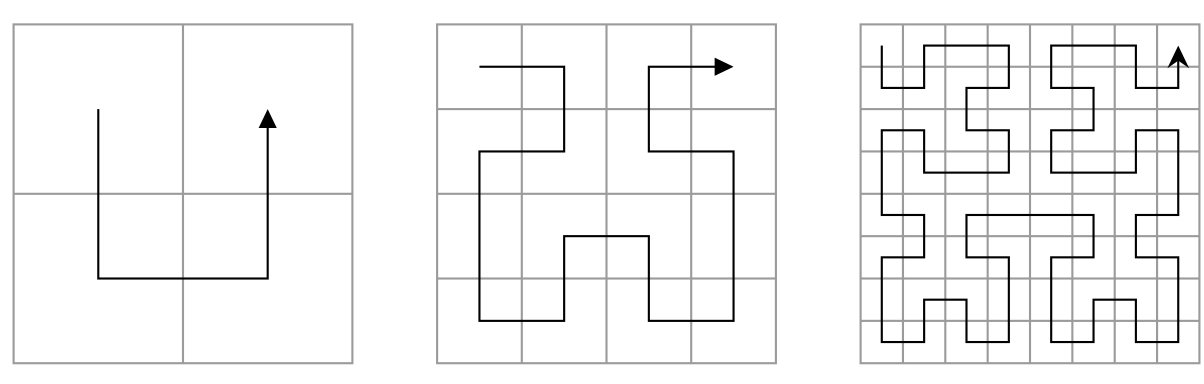
\includegraphics[width=15cm]  {其它/希尔伯特曲线_pic.png}} 
 \end{figure}
\lstinputlisting{其它/希尔伯特曲线.cpp}
\subsection{非整数希尔伯特曲线}
\lstinputlisting{其它/非整数希尔伯特曲线.cpp}
\subsection{约瑟夫环}
\subsubsection{一般方法}
\lstinputlisting{其它/约瑟夫环/一般方法.cpp}
\subsubsection{函数图像解}
\lstinputlisting{其它/约瑟夫环/函数图像解.cpp}


\end{document}